\chapter*{Java应用与开发课程教学体系}

{\kai 很高兴同学门能够选修Java应用与开发课程。

希望我们一起通过这门课程的学习,建立Java语言编程的初步知识体系,掌
握Java应用系统开发的方式、方法。更重要的,能够对编程这个事情、这项技能有
更加深刻的认知,对未来的职业化发展有所促进。

Java应用与开发课程的教学体系如图\ref{fig:java-course-arch}所示,包括
了Java SE和Java EE两个部分,每部分都涉及一些验证性实验,另外,会开展两
次稍微大一点的集成开发项目。同时,在学习的过程中会穿插一些开发工具、设
计模式、应用服务器和数据库的基本应用。

在课程学习的过程中,希望同学们要有足够的求知欲,养成良好的学习态度,具
备不断探索的精神,多尝新、多实践、多总结。我想这是计算机专业人士应该具
备的基本素养。}

\begin{figure}[htb]
\centering
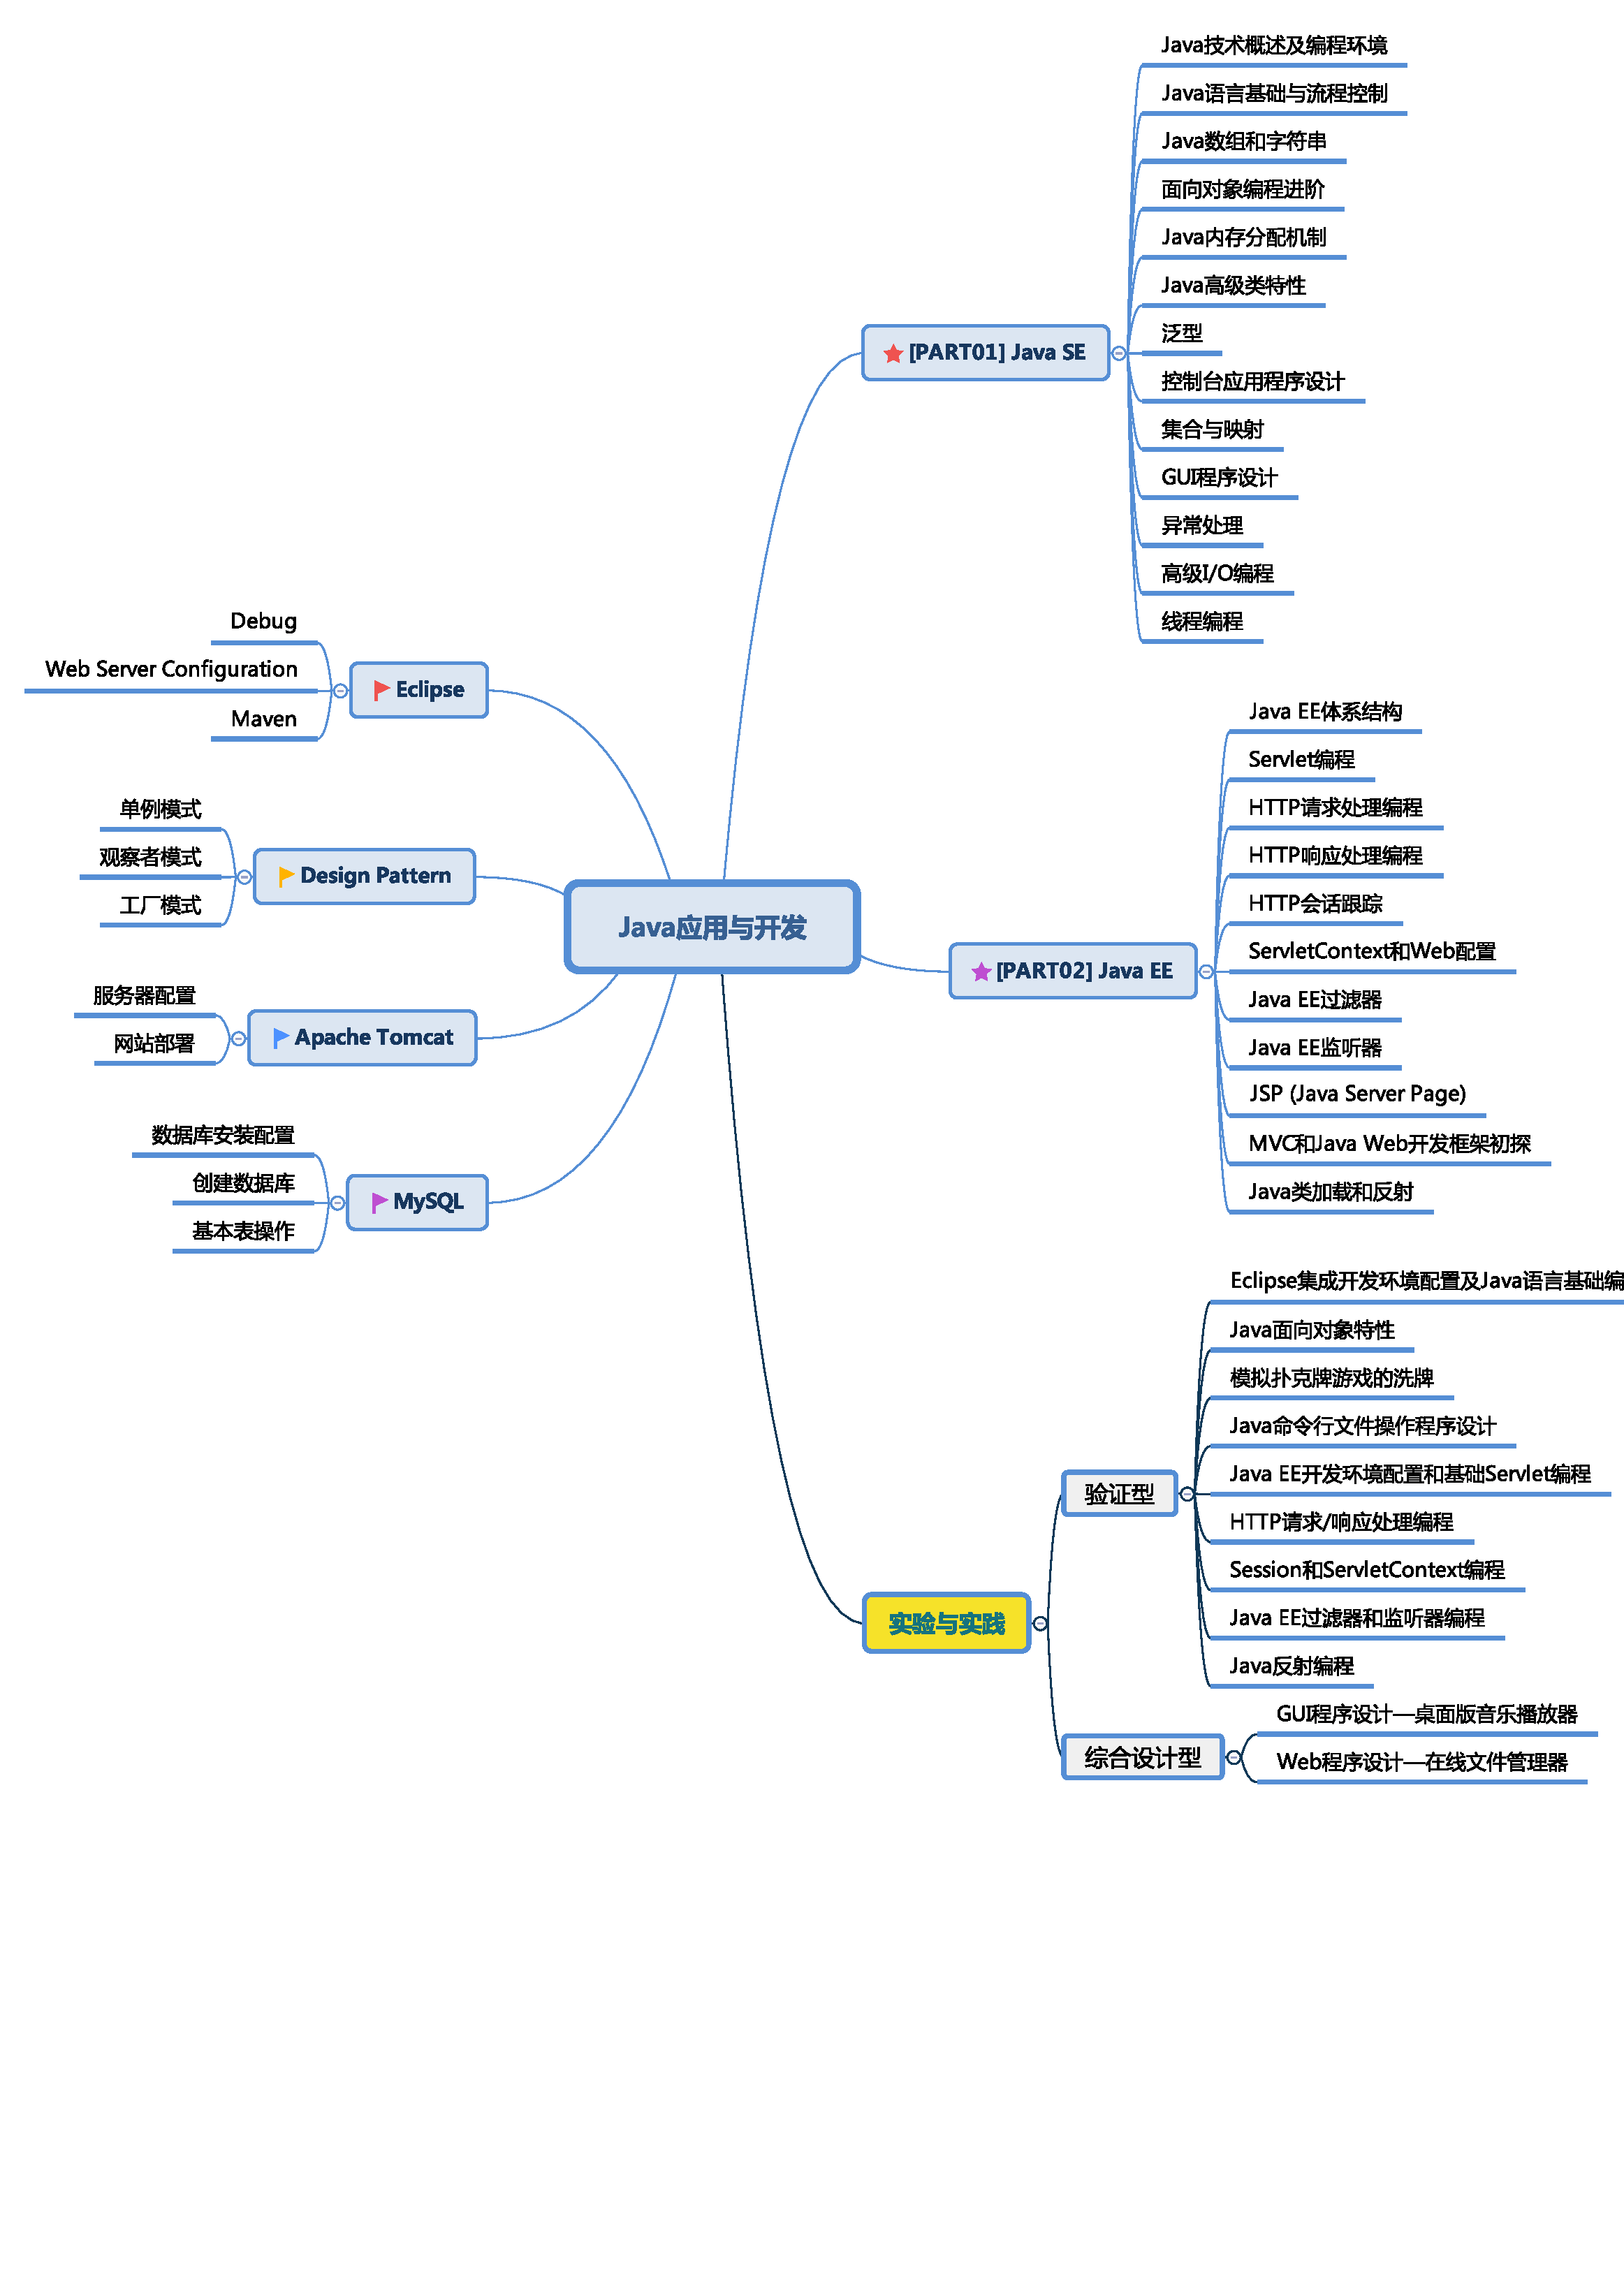
\includegraphics[width=\textwidth]{images/fig-java-course-arch.pdf}
\caption{Java应用与开发课程教学体系}
\label{fig:java-course-arch}
\end{figure}

